\begin{figure}[t]
\vspace{-7em}
\begin{subfigure}[t]{0.45\textwidth}
\centering
    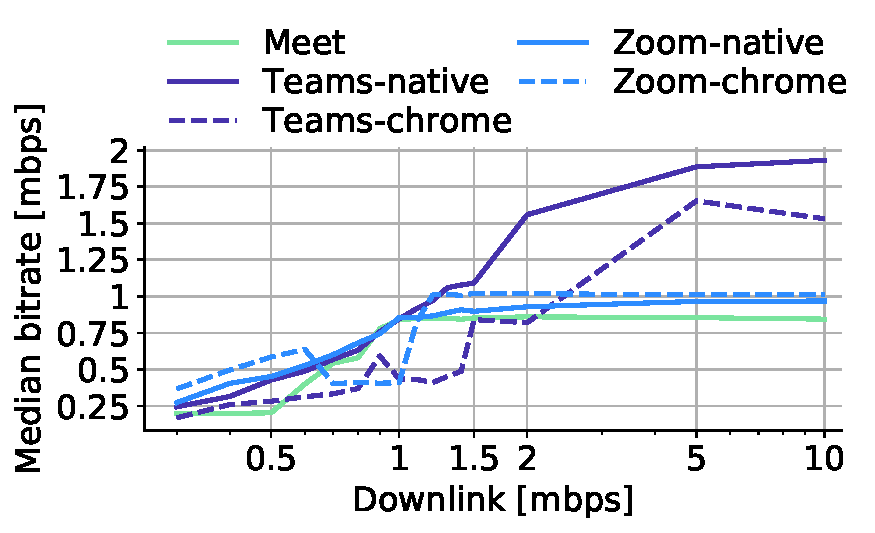
\includegraphics[width=\textwidth,keepaspectratio]{figures/static/downlink.pdf}
    \caption{Downlink bandwidth vs network bitrate}
	\label{subfig:downlink_bitrate}
\end{subfigure} 
\begin{subfigure}[t]{0.45\textwidth}
    \centering
    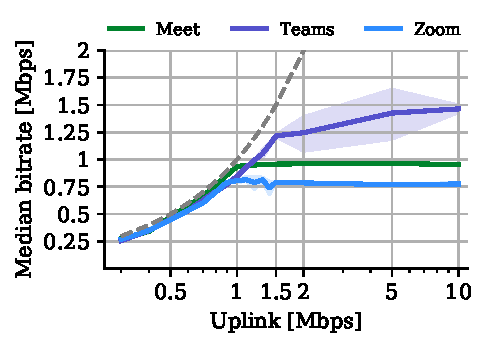
\includegraphics[width=\textwidth,keepaspectratio]{figures/static/uplink.pdf}
    \caption{Uplink bandwidth vs network bitrate}
	\label{subfig:uplink_bitrate}
\end{subfigure}
\caption{Utilization under different link capacities}
\label{fig:static}
\end{figure}

\section{Static Network Conditions}\label{sec:static}

\begin{figure*}[]
	%\vspace{-10em}
    \begin{subfigure}[t]{0.3\textwidth}      
    		\centering
        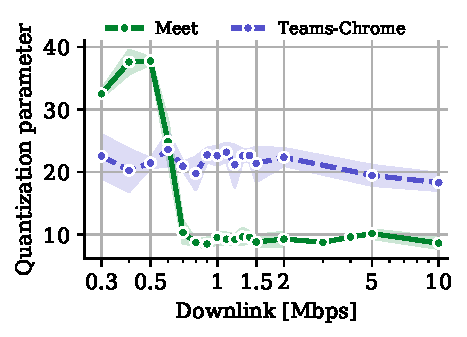
\includegraphics[width=\textwidth,keepaspectratio]{figures/static/downlink_r_qpsum.pdf}
        \vspace{-2em}
        \caption{Quantization parameter}
 		\label{subfig:downlink_video_bitrate}
    \end{subfigure}%
    \hfill
	\begin{subfigure}[t]{0.3\textwidth}   
        \centering
        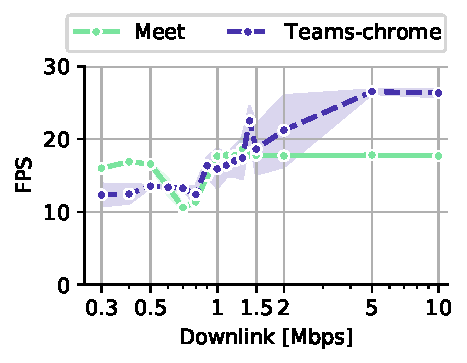
\includegraphics[width=\textwidth]{figures/static/downlink_received_framesPerSecond.pdf}
        \vspace{-2em}
    \caption{Frames per second}
    \label{subfig:downlink_frames_per_second}
    \end{subfigure}% 
    \hfill
	\begin{subfigure}[t]{0.3\textwidth}   
        \centering
        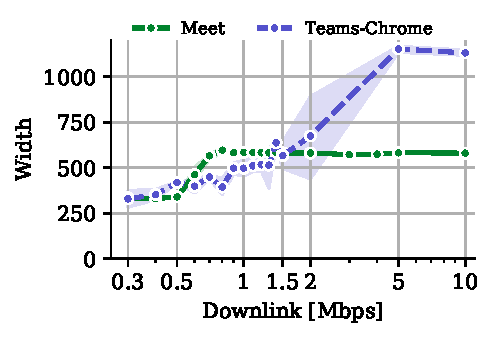
\includegraphics[width=\textwidth]{figures/static/downlink_received_frameWidth.pdf}
        \vspace{-2em}
    \caption{Frame width}
    \label{subfig:downlink_frame_width}
    \end{subfigure}
    \newline
        \begin{subfigure}[t]{0.3\textwidth}      
    		\centering
        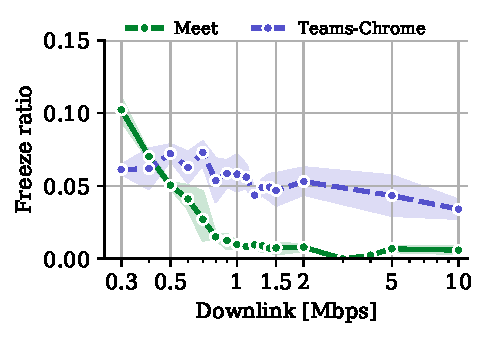
\includegraphics[width=\textwidth,keepaspectratio]{figures/static/downlink_freezeRatio.pdf}
        \vspace{-2em}
        \caption{Freeze ratio}
 		\label{subfig:downlink_freeze_ratio}
    \end{subfigure}%
    \hfill
	\begin{subfigure}[t]{0.3\textwidth}   
        \centering
        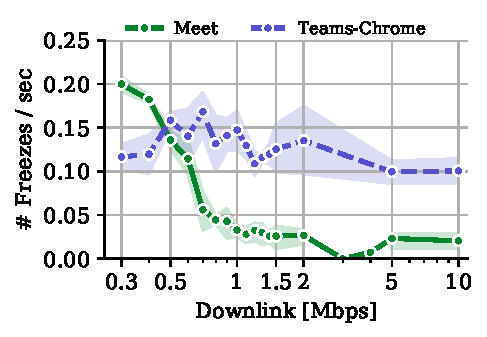
\includegraphics[width=\textwidth]{figures/static/downlink_freezeCountPerSecond.pdf}
        \vspace{-2em}
    \caption{Number of freezes per second}
    \label{subfig:downlink_freeze_per_sec}
    \end{subfigure}% 
    \hfill
	\begin{subfigure}[t]{0.3\textwidth}   
        \centering
        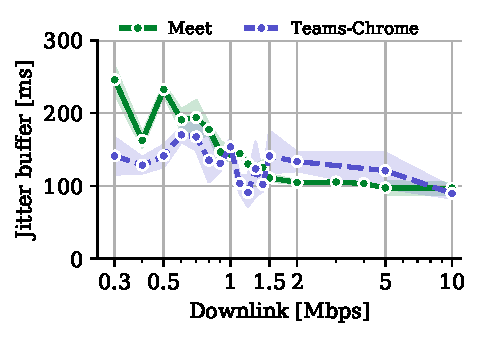
\includegraphics[width=\textwidth]{figures/static/downlink_jitter_buffer.pdf}
        \vspace{-2em}
    \caption{Jitter buffer delay}
    \label{subfig:downlink_jitter_buffer}
    \end{subfigure}
	\vspace{-1em}
	\caption{Downlink bandwidth and application performance metrics}
	\label{fig:downlink_application}
	%\vspace{-1em}
\end{figure*}



In this section, we study the impact of network capacity on the VCA performance. Each experiment consists of a 2.5-minute call between C1 and C2 under a specific shaping level. We conduct two set of experiments with downlink shaped in the first set and uplink shaped in the second set. We consider the following shaping levels: \{$0.3, 0.4, \dots, 1.5, 2, 5, 10$\} Mbps with 5 repetitions at each shaping level.  We also include the browser clients for \zoom and \teams, referred to as \zoombrowser and \teamsbrowser, respectively. This is done to understand if there are any platform-related differences. 
%% experiment setup
%% what is the experiment duration 
%% what bandwidth profiles are used 

% \tarun{Open questions: i) What about Team native client? ii) Audio performance? iii) Re-do \zoombrowser for 0.3 Mbps and 0.4 Mbps}



\subsection{Impact on network data rate} Figure~\ref{fig:downlink_bitrate} shows the median received network bitrate averaged over 5 runs for different downlink shaping levels. We find differences among VCAs in terms of their bitrate configuration and bitrate adaptation leading to different performance under same network conditions. For instance, the peak utilization for \teamsnative is $1.9$ Mbps whereas it is only $0.96$ for \zoomnative and $0.8$ Mbps for \meet. The received bitrate also reflects how different VCAs utilize the network especially under constrained links. Interestingly, we find that \zoomnative has the highest network utilization while \meet has the lowest (only $50\%$ at 0.5 Mbps) for downlink capacity lower than 0.75 Mbps. Finally, we also observe differences between \teamsbrowser and \teamsnative under same network conditions with the former having lower bitrates than the latter. For instance, at 1 Mbps shaping level, the received bitrate is only 0.5 Mbps for \teamsbrowser and 0.8 Mbps for \teamsnative. This suggests that implementation of the VCA can differ across platforms leading to different network and application behavior. 

\begin{figure}[t]
	%\vspace{-1em}
    \begin{subfigure}[t]{0.23\textwidth}      
    		\centering
        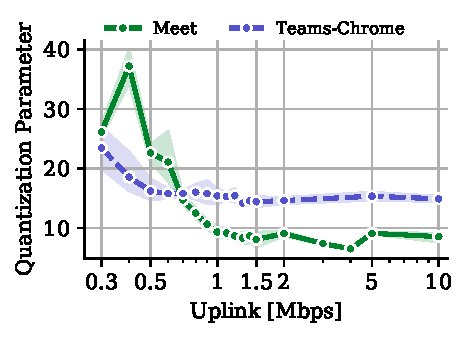
\includegraphics[width=\textwidth,keepaspectratio]{figures/static/uplink_s_qpsum.pdf}
        \vspace{-2em}
        \caption{Quantization parameter}
 		\label{subfig:uplink_video_quantization}
    \end{subfigure}%
\hfill
	\begin{subfigure}[t]{0.23\textwidth}   
        \centering
        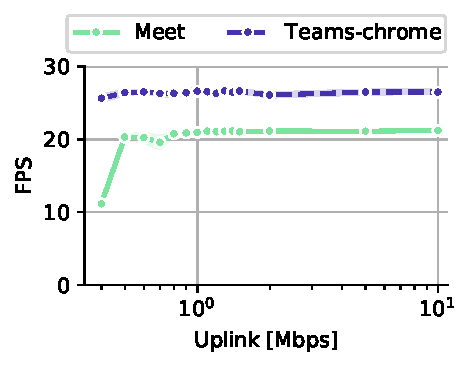
\includegraphics[width=\textwidth]{figures/static/uplink_sent_framesPerSecond.pdf}
        \vspace{-2em}
    \caption{Frames per second}
    \label{subfig:uplink_frames_per_second}
    \end{subfigure}% 
        \newline
    \hfill
	\begin{subfigure}[t]{0.23\textwidth}   
        \centering
        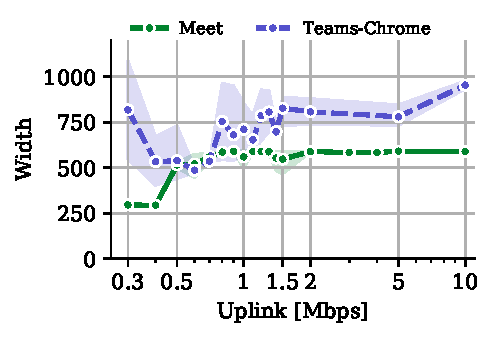
\includegraphics[width=\textwidth]{figures/static/uplink_sent_frameWidth.pdf}
        \vspace{-2em}
    \caption{Frame width}
    \label{subfig:uplink_frame_width}
    \end{subfigure}
        \begin{subfigure}[t]{0.23\textwidth}      
    		\centering
        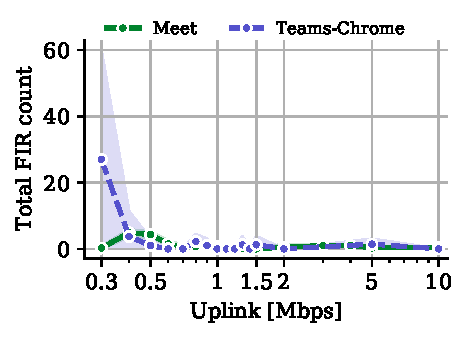
\includegraphics[width=\textwidth,keepaspectratio]{figures/static/uplink_sent_firCount.pdf}
        \vspace{-2em}
        \caption{FIR Count}
 		\label{subfig:uplink_fir}
    \end{subfigure}%
	\vspace{-1em}
	\caption{Uplink bandwidth and application performance metrics}
	\label{fig:uplink_application}
	%\vspace{-1em}
\end{figure}


\begin{table}[]
\centering
\begin{tabular}{|c|c|c|}
\hline
\textbf{VCA} & \textbf{\begin{tabular}[c]{@{}c@{}}Nominal bitrate \\ (Mbps)\end{tabular}} & \textbf{\begin{tabular}[c]{@{}c@{}}Observed \\ resolutions\end{tabular}} \\ \hline
\hline 
Meet         & 0.8                                                                        & x                                                                        \\ \hline
Teams        & 1.96 Mbps                                                                  & x                                                                        \\ \hline
Zoom         & 0.95 Mbps                                                                  & x                                                                        \\ \hline
\end{tabular}
\caption{Bitrate and resolutions for the VCAs}
\label{tab:vca_static}
\end{table}

\begin{figure*}[h!]
\begin{subfigure}[t]{.5\textwidth}
    \centering
    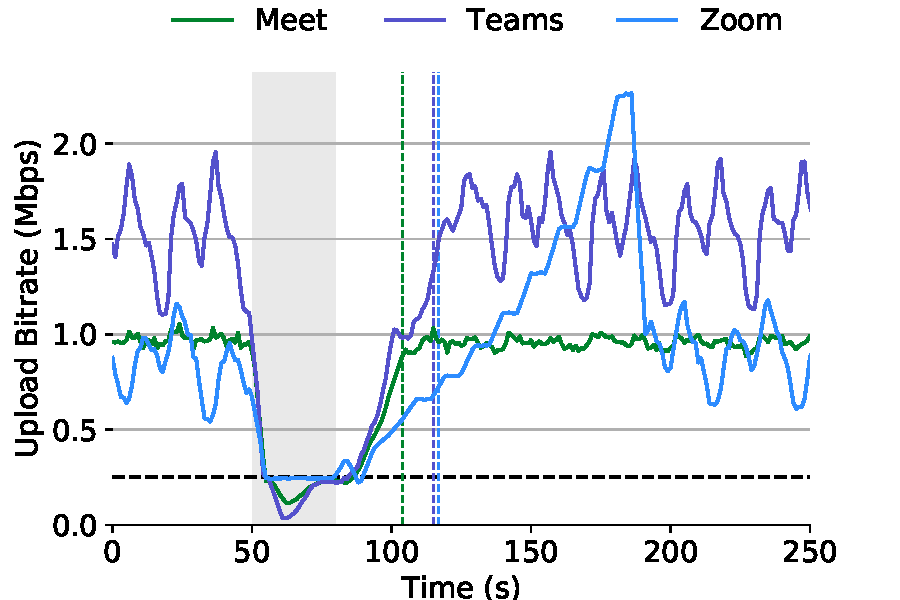
\includegraphics[width=\textwidth,keepaspectratio]{interrupt/Interrupt-upld.pdf}
    \captionsetup{width=.9\linewidth}
    \caption{Average uplink bitrate over time. Grey region indicates period where uplink capacity is constrained to 0.25 Mbps. Vertical dotted lines indicate when the uplink bitrate has returned to the average. Dotted horizontal line indicates the uplink shaping level.}
    \label{fig:ts_upld}
\end{subfigure}\hfill
\begin{subfigure}[t]{.5\textwidth}
      \centering
    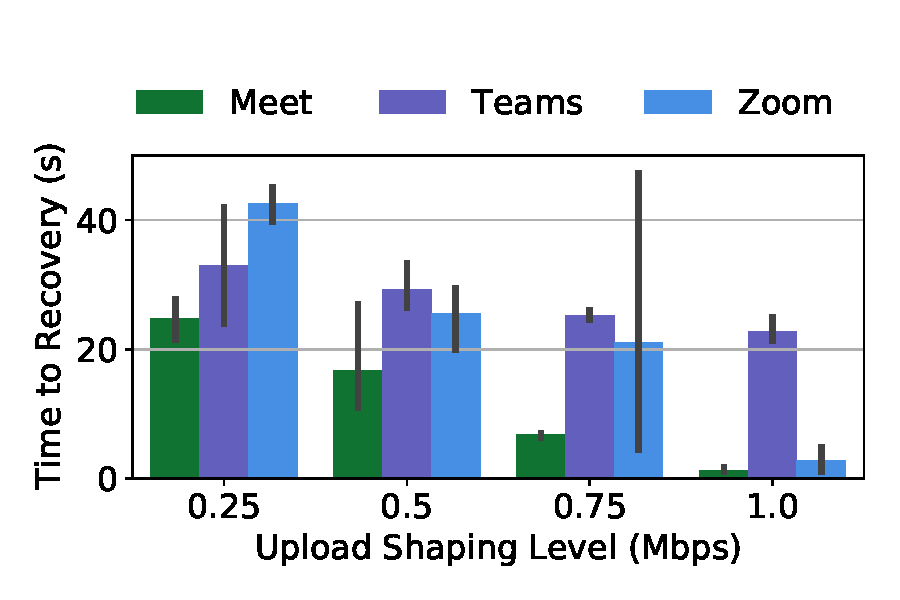
\includegraphics[width=1\textwidth,keepaspectratio]{interrupt/TTR-upld.pdf}
    \captionsetup{width=.9\linewidth}
    \caption{The time to recover to average sending bitrate following a drop to the indicated uplink shaping level}
    \label{fig:TTR_upld}
\end{subfigure}
\caption{VCA response to a 30s drop in available uplink capacity}
\label{fig:interrupt-upld}
\end{figure*}


We next analyze the median sent network bitrate for different uplink capacity (see Figure~\ref{fig:uplink_bitrate}). As expected, we find similar differences in terms of the maximum bitrate among the VCAs and between browser and native clients for \teams as observed in the downlink shaping experiment. However, the network utilization is higher, especially for \meet, when the upstream link is constrained as compared to downlink. Thus, there seems to be a discrepancy in bitrate adaptation when the upstream is constrained. We explore this discrepancy in more detail in Section~\ref{sec:interruption}. 

\subsection{Impact on application performance}
Here we describe how the link shaping level impacts application performance metrics. However, obtaining application metrics can be challenging for VCAs. We rely on WebRTC stats available on Google Chrome to obtain statistics for \teamsbrowser and \meet. We could not obtain the same statistics for \zoombrowser as it used different transport channels to transmit media, i.e., datachannels instead of the RTP MediaStream~\cite{webrtc_stats} as it may provides more flexibility (e.g., flexible encoding standards) to \zoom. However, video quality statistics are not exposed anymore through the WebRTC stats API. %In addition, we also obtained access to Zoom API through our campus network operator. The Zoom API provides limited application performance (e.g., video resolution, FPS) at a per-minute granularity~\cite{zoom_qos_api}. 
Thus, we limit this analysis to only \meet and \teamsbrowser for this section. 

%More specifically, we consider the following application metrics: Frames per second, video resolution, freeze ratio. 





\textbf{Application metrics and bitrate adaptation}: VCAs can ideally adapt the video bitrate by adjusting one or more of the following three parameters: i) frames per second (\textit{FPS}), ii) \textit{quantization parameter} used in image compression, and  iii) \textit{video resolution} indicating the number of pixels in each dimension. We indicate resolution with one of the dimension, i.e., \textit{frame width} in our analysis. Figure~\ref{fig:downlink_application} shows the above parameters for \meet and \teamsbrowser under different downlink shaping levels. 




We find that \teamsbrowser simultaneously degrades all three parameters as the downlink becomes more constrained. There is also significant variance across multiple repetitions under the same network bandwidth as shown by the $90\%$ confidence interval bands in the plot. \meet, on the other hand, follows a more consistent trend. In the 0.7-1 Mbps region, the bitrate is controlled mostly by adapting the FPS while keeping the quantization parameter and frame width similar to the nominal levels. However, after 0.7 Mbps, both \textit{resolution} and \textit{quantization parameter} degrade whereas there is an increase in the FPS. Below 0.5 Mbps, the frame width and the FPS stabilize while the quantization parameter actually reduces. It is not clear as to why \meet chose to reduce the quantization parameter after 0.5 Mbps and increase the FPS after 0.8 Mbps. 

We also plot the statistics related to video freezes during the call as obtained from the WebRTC stats. A freeze is assumed to occur if the frame inter-arrival is either greater than 3 $\times$ average frame duration or $150 ms$ + average frame duration.  Figure~\ref{subfig:downlink_freeze_ratio} and~\ref{subfig:downlink_freeze_per_sec} show the freeze ratio and number of freezes per second for \meet and \teamsbrowser. We find that both freeze ratio and freezes per second increase as the downlink bandwidth degrades. For \meet, the degradation is more severe than \teamsbrowser with $10\%$ freeze ratio at 0.3 Mbps. 


% Figure~\ref{fig:down}



\textbf{Takeaway}: VCA performance under same network conditions varies.  
%% also plot differences in network utilization and the shaping. 



%% Difference among VCAs. Peak utlization differs. For the same network conditions, VCAs peform differently. For instance, Teams on WebRTC 
%% Difference between native and browser client 
%% Google Meet Simulcast





\begin{comment}
\begin{figure}[t]
    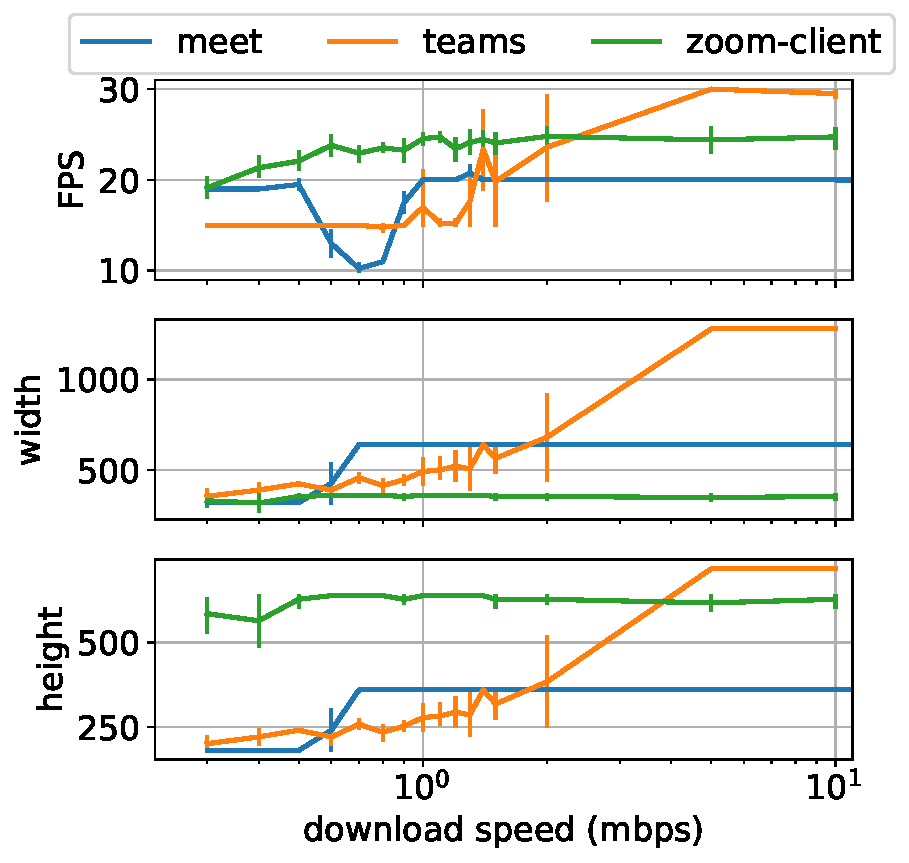
\includegraphics[width=0.35\textwidth,keepaspectratio]{figures/static/downlink_video_qual_meet_teams_zoom.pdf}
    \caption{Downlink bandwidth vs video quality \jamie{I think that width and height are almost always exactly redundant information.  I would choose one.  We should also keep the same colors across plots -- blue shouldn't be both Meet and Zoom client, for instance.}}
    \label{fig:downlink_video_qual}
\end{figure}


\begin{figure}[t]
    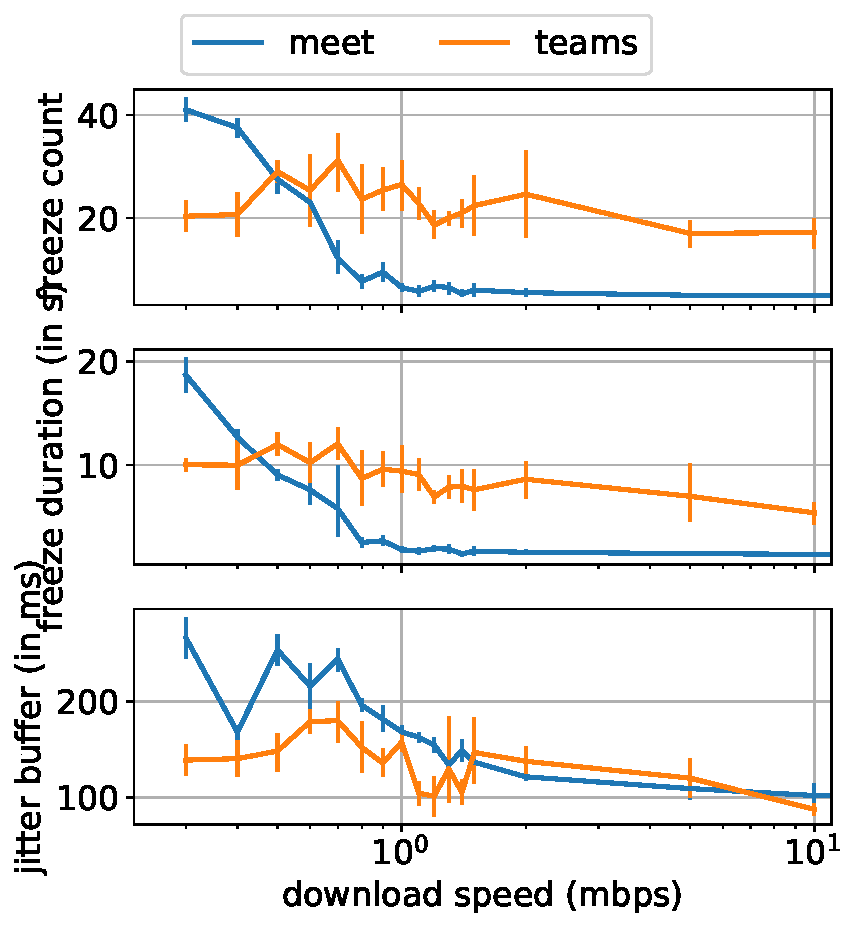
\includegraphics[width=0.35\textwidth,keepaspectratio]{figures/static/downlink_freeze_meet_teams.pdf}
    \caption{Downlink bandwidth and video freezes}
    \label{fig:downlink_freeze}
\end{figure}



\begin{figure}[t]
    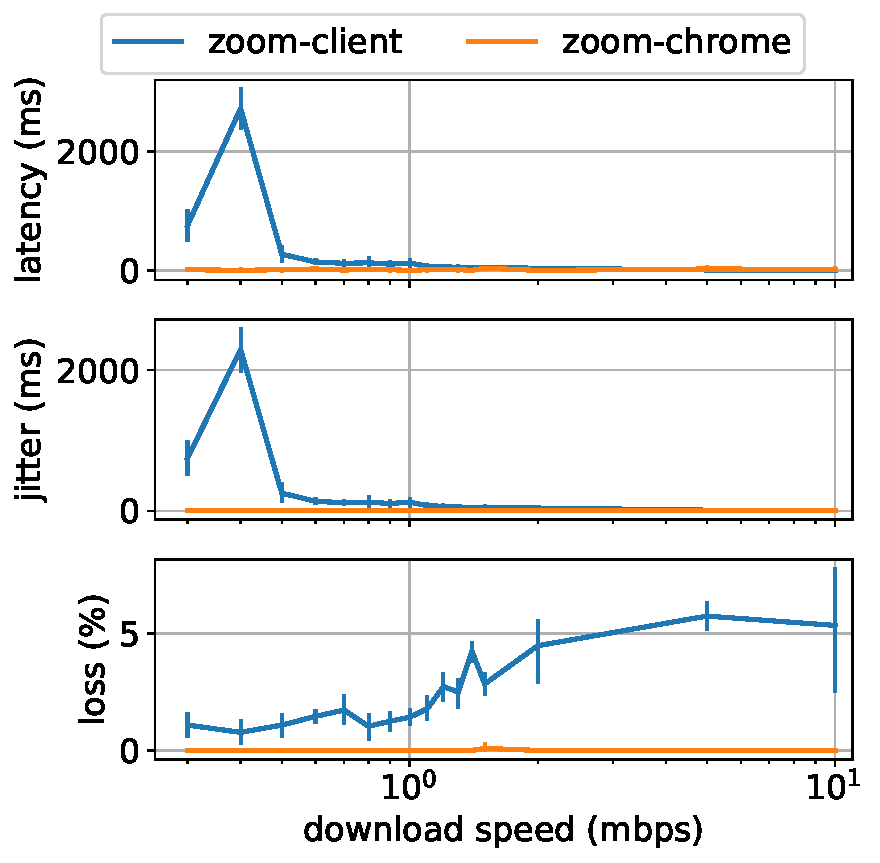
\includegraphics[width=0.35\textwidth,keepaspectratio]{figures/static/downlink_qos_zoom.pdf}
    \caption{Downlink bandwidth vs Zoom QoS. \jamie{It looks fishy, that zoom client latency and jitter are identical.  All data from browser seems to be zeroed out?}} 
    \label{fig:downlink_qos_zoom}
\end{figure}
\end{comment}